38. $y=\cfrac{(x+1)(x-3)}{|x-1|+2}=\begin{cases} \cfrac{(x+1)(x-3)}{x-1+2},\ x\geqslant1,\\ \cfrac{(x+1)(x-3)}{1-x+2},\ x<1.\end{cases}=
\begin{cases} x-3,\ x\geqslant1,\\ -x-1,\ x<1.\end{cases}$
$$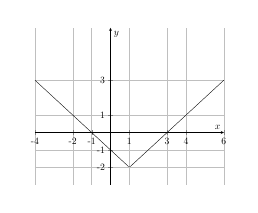
\begin{tikzpicture}[scale=0.35]
\begin{axis}[
    axis lines = middle,
    grid=major,
    legend pos={south west},
    xlabel = {$x$},
    ylabel = {$y$},
    ymin=-3,
    ymax=6,
    xtick={ -4, -1, 1, 4,3, 6,-2},
    xticklabels={ -4, -1, 1, 4,3, 6,-2},
    ytick={ -2, 1, -1,3},
    yticklabels={ -2, 1, -1,3}            ]
	\addplot[domain=-4:6, samples=100, color=black] {(x+1)*(x-3)/(abs(x-1)+2)};
%\addplot[domain=-3.1:2.5, samples=100, color=red] {70*abs(1-2*abs(abs(x)-2))-10*x^2+10*x-70};
	%\addlegendentry{$\text{Рис. 1}$};
\end{axis}
\end{tikzpicture}$$
